\chapter{Introduction}

More than 200 years after Isaac Newton defined the law of universal gravitation, Albert Einstein drastically changed humanity's understanding of gravity with the theory of General Relativity. Gravity was no longer a force in the traditional sense, instead it had to be viewed as a manifestation of curved spacetime. In this new theory, matter and energy influence the coordinates of spacetime around them, resulting in Einstein's nonlinear field equations. The field equations of General Relativity are immensely difficult to solve in any situation without great symmetry, but their predictions have been repeatedly proven correct since Einstein introduced them in 1915~\cite{einstein1916naherungsweise}. Specific tests of General Relativity include the perihelion precession of Mercury, the deflection of light by the sun, and the gravitational redshift of light. The results of these tests brought Einstein's theory to the forefront of physics.

Gravitational Waves (GWs) are ripples in spacetime that propagate at the speed of light. The possibility was first theorized all the way back in 1893 by Oliver Heaviside with use of analogies to electricity~\cite{heaviside1893gravitational}. In 1905, Henri Poincar\'e proposed that GWs could be emitted from accelerated bodies and should propagate at the speed of light, as required by Lorentz transformations~\cite{goldberg1967henri}. Einstein was doubtful about the existence of GWs due to the lack of gravitational dipoles, but he did pursue the topic. In 1936 Einstein attempted to publish a paper with Nathan Rosen claiming that GWs could not in fact exist because they would require singularities. A reviewer of the paper, Howard P. Robertson, eventually convinced him that these singularities were in fact entirely due to his use of cylindrical coordinates. It wasn't until 1981 that strong evidence for GWs emerged due to analysis of the Hulse-Taylor puslar~\cite{weisberg1981gravitational}. This pulsar orbits another neutron star in a binary system and the orbital period has been shown to decrease at the expected rate due to GW emission.

Efforts to directly observe GWs began with Joseph Weber in the 1960s. He created devices known as Weber bars that contained multiple large aluminum cylinders designed to vibrate at a resonant frequency when a GW passed by. Despite his many claims of detections~\cite{weber1969evidence}, these results were eventually shown to be incorrect. The first direct observation of a GW occured in 2015 by the Laser Interferometer Gravitational Wave Observatory (LIGO) collaboration~\cite{GW150914}. Spectrograms of the signal can be seen in Figure~\ref{fig:GW150914}. LIGO consists of two 4\,km long interferometers located in Hanford, WA and Livingston, LA. The GW observed, GW150914, originated from two orbiting black holes and travelled towards Earth for over a billion years. Two years later, the detection of GW170817 initiated multi-messenger astronomy as it was accompanied by a gamma-ray burst (GRB)~\cite{GW170817}. 

\begin{figure*}[b!]
    \centering
    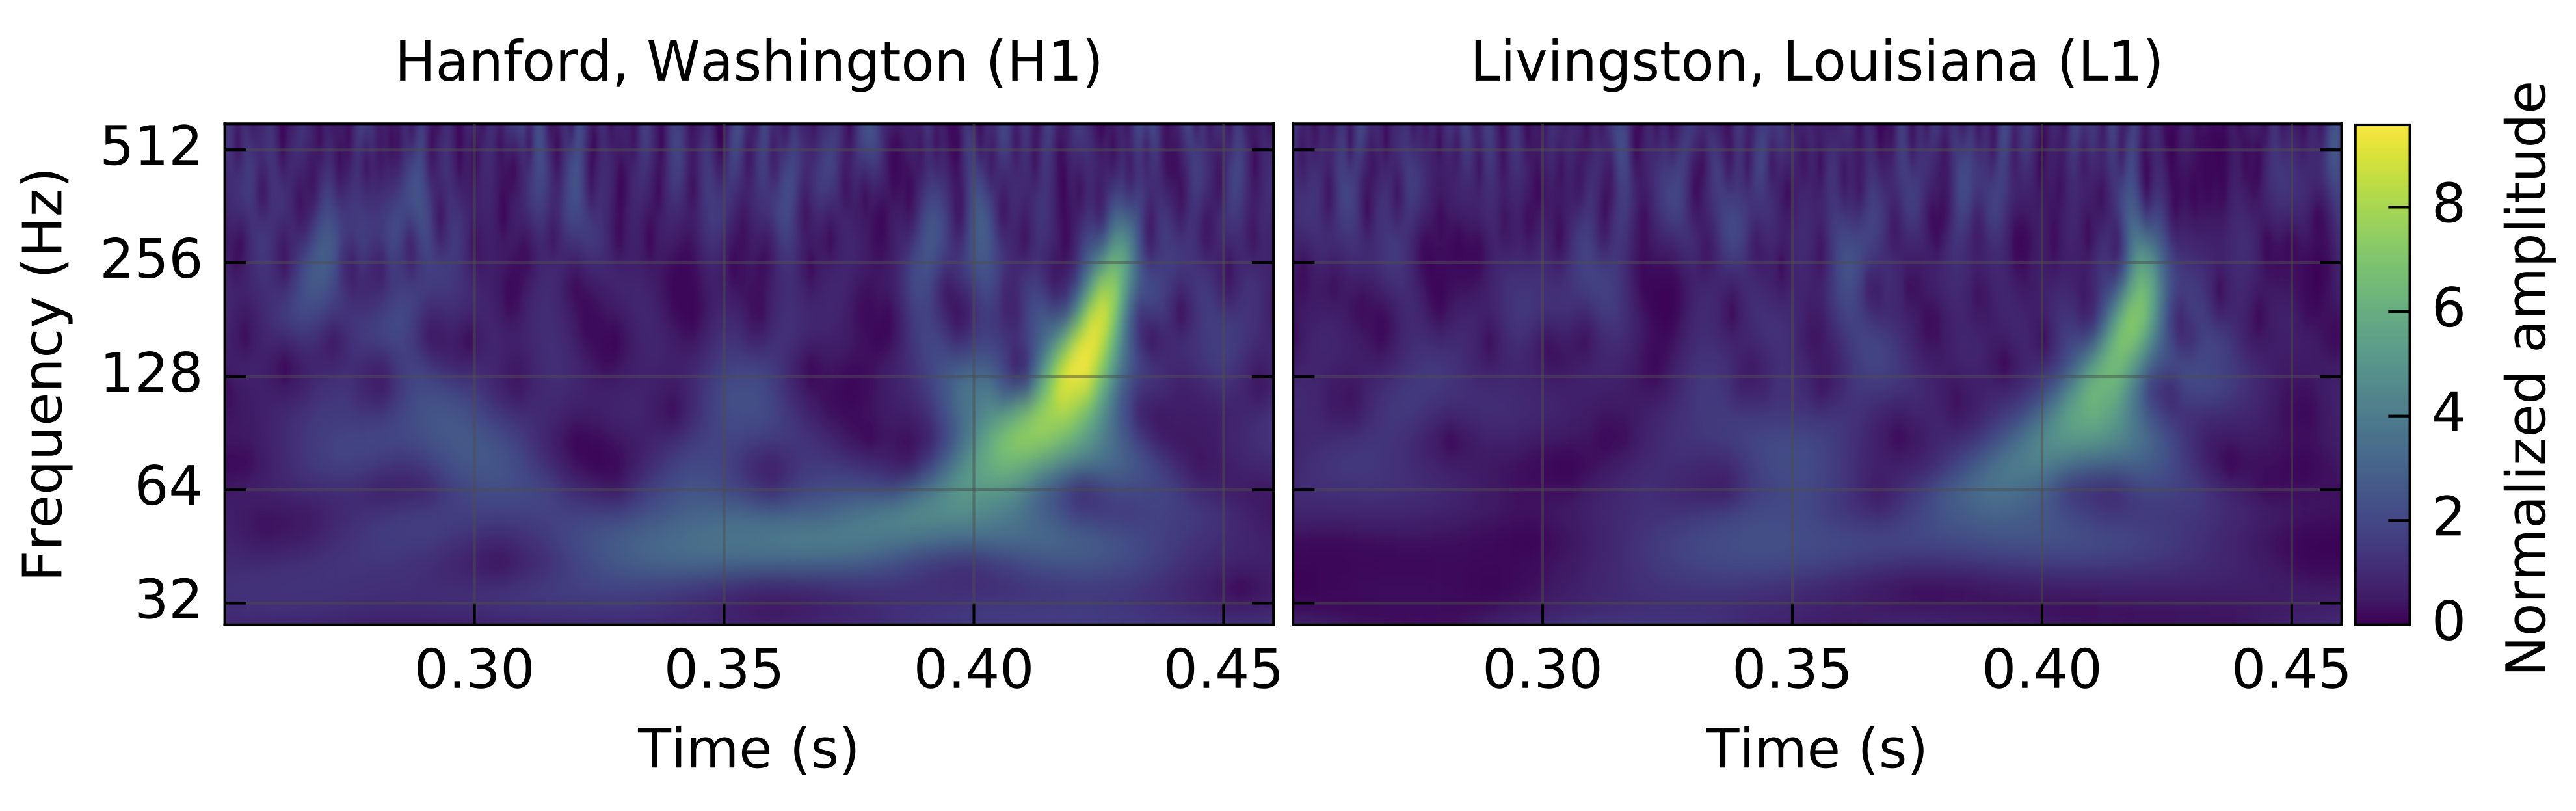
\includegraphics[width=\textwidth]{figures/GW150914.png}
    \caption{Spectrograms of GW150914, the first GW ever observed~\cite{GW150914}.}
    \label{fig:GW150914}
\end{figure*}

GW observations have already resulted in three Nobel Prizes being awarded to LIGO-affiliated physicists. So far every GW detection has originated from a compact binary system, but there are many other objects predicted to be sources of GWs. Core-collapse supernovae (CCSNe) represent one of the most promising sources of GWs yet to be observed. CCSNe can shine brightly for days, weeks, or months at a time and have been observed in the sky for thousands of years. They are also believed to be essential to our existence and way of life as they are instrumental to the spread of heavy metals throughout the universe. Despite this, the details and underlying physcis of a CCSN explosion are still somewhat mysterious. Most simulations fail to explode and there is significant uncertainty about the mechanisms and processes at work within the star in its final moments. GWs are emitted from the core of a CCSN, as opposed to electromagnetic radiation which is emitted only from the outermost layers. GWs therefore offer a unique glimpse into the heart of the star and could help physicists understand the nuclear equation of state present in a neutron star. Unfortunately, CCSNe are rare and emit weaker GWs than compact binary systems. The chances of a GW observation from a CCSN will therefore increase over the next few decades as detector sensitivities improve.

The first GW observed from a CCSN will be an important moment in astrophysics. In order to learn something from such an event, parameter estimation tools and algorithms must be developed. GWs from CCSNe are inherently random. This, in combination with the uncertainty of the underlying physics, makes parameter estimation a difficult task. This dissertation will cover my work with the LIGO collaboration with a focus on the Supernova Model Evidence Extractor (SMEE), a working parameter estimation tool for GWs from CCSNe. Chapter~\ref{GWs} will cover GWs and GW detectors. Chapter~\ref{chp:pem} will cover my work with LIGO's Physical Environment Monitoring (PEM) system. Chapter~\ref{chp:CCSNe} will cover CCSNe and their numerical relativity simulations. Chapter~\ref{chp:SMEE} will describe the SMEE algorithm in great detail, and chapter~\ref{chp:performance} will outline the performance of SMEE with an emphasis on future detectors. 